\documentclass[tikz, border=6pt]{standalone}

\usepackage{amsmath,amssymb}
\usepackage{pgfplots}
\pgfplotsset{compat=1.18}
\usepgfplotslibrary{groupplots}
\usetikzlibrary{arrows.meta}
\usepackage{xcolor}

\definecolor{utnblue}{RGB}{0, 51, 102}

% Franja gris sobre los k que la ventana cubre en el instante #1:
% h[n-k] es no nula desde k=n-3 hasta k=n.
\newcommand{\ventana}[3]{%
    \fill[black!8] (axis cs:{#1-3.45},#2) rectangle (axis cs:{#1+0.45},#3);}

% Rotulo de fila, al margen izquierdo del primer panel de cada fila.
\newcommand{\filalabel}[1]{%
    \node[anchor=east, font=\scriptsize, inner sep=0pt]
        at (axis description cs:-0.04,0.5) {#1};}

\begin{document}
    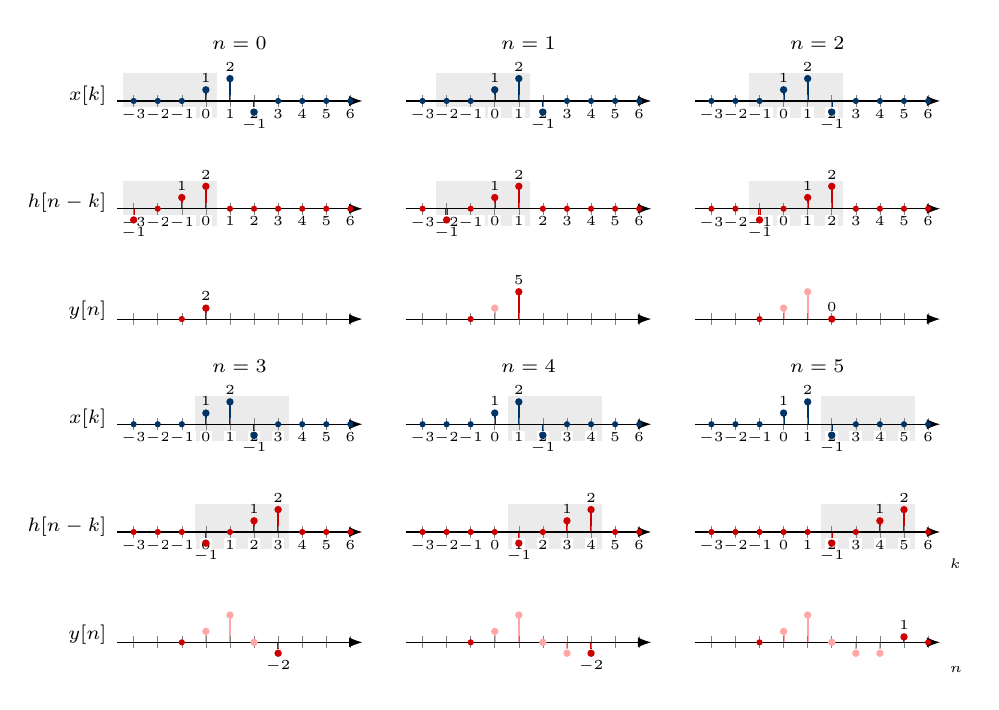
\begin{tikzpicture}[>=Latex, font=\scriptsize]
        \begin{groupplot}[
            group style={group size=3 by 6,
                         horizontal sep=0.55cm, vertical sep=0.80cm},
            width=4.7cm, height=2.15cm,
            axis x line=middle, axis y line=none,
            axis line style={->, thin, black},
            xmin=-3.7, xmax=6.5,
            xtick={-3,-2,-1,0,1,2,3,4,5,6},
            every tick label/.style={font=\tiny, fill=white, inner sep=0.6pt},
            title style={font=\scriptsize, yshift=-1pt},
            nodes near coords, point meta=explicit symbolic,
            every node near coord/.style={font=\tiny, text=black, anchor=south,
                                          inner sep=1.2pt, yshift=1pt},
            entrada/.style={ycomb, mark=*, mark size=0.9pt, thick, utnblue},
            resimp/.style={ycomb, mark=*, mark size=0.9pt, thick, red!80!black},
            salida/.style={ycomb, mark=*, mark size=0.9pt, thick, red!80!black},
            ceroent/.style={only marks, mark=*, mark size=0.9pt, utnblue,
                            point meta=none, nodes near coords={}},
            cerores/.style={only marks, mark=*, mark size=0.9pt, red!80!black,
                            point meta=none, nodes near coords={}},
            previa/.style={ycomb, mark=*, mark size=0.9pt, thick, red!35!white,
                           point meta=none, nodes near coords={}},
            rotuloabajo/.style={every node near coord/.style={font=\tiny,
                                text=black, anchor=north, inner sep=1.2pt,
                                yshift=-1pt}},
            escent/.style={ymin=-1.5, ymax=2.5},
            escsal/.style={ymin=-2.6, ymax=5.6, xticklabels={}},
            axis on top,
            clip=false,
        ]
        % =====================================================================
        % BLOQUE 1 --- instantes n=0, n=1, n=2
        % =====================================================================
        % ---- fila 1: la entrada x[k] ----
        \nextgroupplot[escent, title={$n=0$}]
            \filalabel{$x[k]$}
            \ventana{0}{-1.5}{2.5}
            \addplot[entrada] coordinates {(0,1) [$1$] (1,2) [$2$]};
            \addplot[entrada, rotuloabajo] coordinates {(2,-1) [$-1$]};
            \addplot[ceroent] coordinates {(-3,0) (-2,0) (-1,0) (3,0) (4,0) (5,0) (6,0)};
        \nextgroupplot[escent, title={$n=1$}]
            \ventana{1}{-1.5}{2.5}
            \addplot[entrada] coordinates {(0,1) [$1$] (1,2) [$2$]};
            \addplot[entrada, rotuloabajo] coordinates {(2,-1) [$-1$]};
            \addplot[ceroent] coordinates {(-3,0) (-2,0) (-1,0) (3,0) (4,0) (5,0) (6,0)};
        \nextgroupplot[escent, title={$n=2$}]
            \ventana{2}{-1.5}{2.5}
            \addplot[entrada] coordinates {(0,1) [$1$] (1,2) [$2$]};
            \addplot[entrada, rotuloabajo] coordinates {(2,-1) [$-1$]};
            \addplot[ceroent] coordinates {(-3,0) (-2,0) (-1,0) (3,0) (4,0) (5,0) (6,0)};

        % ---- fila 2: los pesos h[n-k] ----
        \nextgroupplot[escent]
            \filalabel{$h[n-k]$}
            \ventana{0}{-1.5}{2.5}
            \addplot[resimp] coordinates {(-1,1) [$1$] (0,2) [$2$]};
            \addplot[resimp, rotuloabajo] coordinates {(-3,-1) [$-1$]};
            \addplot[cerores] coordinates {(-2,0) (1,0) (2,0) (3,0) (4,0) (5,0) (6,0)};
        \nextgroupplot[escent]
            \ventana{1}{-1.5}{2.5}
            \addplot[resimp] coordinates {(0,1) [$1$] (1,2) [$2$]};
            \addplot[resimp, rotuloabajo] coordinates {(-2,-1) [$-1$]};
            \addplot[cerores] coordinates {(-3,0) (-1,0) (2,0) (3,0) (4,0) (5,0) (6,0)};
        \nextgroupplot[escent]
            \ventana{2}{-1.5}{2.5}
            \addplot[resimp] coordinates {(1,1) [$1$] (2,2) [$2$]};
            \addplot[resimp, rotuloabajo] coordinates {(-1,-1) [$-1$]};
            \addplot[cerores] coordinates {(-3,0) (-2,0) (0,0) (3,0) (4,0) (5,0) (6,0)};

        % ---- fila 3: la salida y[n] ----
        \nextgroupplot[escsal]
            \filalabel{$y[n]$}
            \addplot[salida] coordinates {(0,2) [$2$]};
            \addplot[cerores] coordinates {(-1,0)};
        \nextgroupplot[escsal]
            \addplot[previa] coordinates {(0,2)};
            \addplot[salida] coordinates {(1,5) [$5$]};
            \addplot[cerores] coordinates {(-1,0)};
        \nextgroupplot[escsal]
            \addplot[previa] coordinates {(0,2) (1,5)};
            \addplot[salida] coordinates {(2,0) [$0$]};
            \addplot[cerores] coordinates {(-1,0)};

        % =====================================================================
        % BLOQUE 2 --- instantes n=3, n=4, n=5
        % =====================================================================
        % ---- fila 4: la entrada x[k] ----
        \nextgroupplot[escent, title={$n=3$}]
            \filalabel{$x[k]$}
            \ventana{3}{-1.5}{2.5}
            \addplot[entrada] coordinates {(0,1) [$1$] (1,2) [$2$]};
            \addplot[entrada, rotuloabajo] coordinates {(2,-1) [$-1$]};
            \addplot[ceroent] coordinates {(-3,0) (-2,0) (-1,0) (3,0) (4,0) (5,0) (6,0)};
        \nextgroupplot[escent, title={$n=4$}]
            \ventana{4}{-1.5}{2.5}
            \addplot[entrada] coordinates {(0,1) [$1$] (1,2) [$2$]};
            \addplot[entrada, rotuloabajo] coordinates {(2,-1) [$-1$]};
            \addplot[ceroent] coordinates {(-3,0) (-2,0) (-1,0) (3,0) (4,0) (5,0) (6,0)};
        \nextgroupplot[escent, title={$n=5$}]
            \ventana{5}{-1.5}{2.5}
            \addplot[entrada] coordinates {(0,1) [$1$] (1,2) [$2$]};
            \addplot[entrada, rotuloabajo] coordinates {(2,-1) [$-1$]};
            \addplot[ceroent] coordinates {(-3,0) (-2,0) (-1,0) (3,0) (4,0) (5,0) (6,0)};

        % ---- fila 5: los pesos h[n-k] ----
        \nextgroupplot[escent]
            \filalabel{$h[n-k]$}
            \ventana{3}{-1.5}{2.5}
            \addplot[resimp] coordinates {(2,1) [$1$] (3,2) [$2$]};
            \addplot[resimp, rotuloabajo] coordinates {(0,-1) [$-1$]};
            \addplot[cerores] coordinates {(-3,0) (-2,0) (-1,0) (1,0) (4,0) (5,0) (6,0)};
        \nextgroupplot[escent]
            \ventana{4}{-1.5}{2.5}
            \addplot[resimp] coordinates {(3,1) [$1$] (4,2) [$2$]};
            \addplot[resimp, rotuloabajo] coordinates {(1,-1) [$-1$]};
            \addplot[cerores] coordinates {(-3,0) (-2,0) (-1,0) (0,0) (2,0) (5,0) (6,0)};
        \nextgroupplot[escent, xlabel={$k$},
                       xlabel style={anchor=north west, at={(axis description cs:1,0)}, font=\tiny}]
            \ventana{5}{-1.5}{2.5}
            \addplot[resimp] coordinates {(4,1) [$1$] (5,2) [$2$]};
            \addplot[resimp, rotuloabajo] coordinates {(2,-1) [$-1$]};
            \addplot[cerores] coordinates {(-3,0) (-2,0) (-1,0) (0,0) (1,0) (3,0) (6,0)};

        % ---- fila 6: la salida y[n] ----
        \nextgroupplot[escsal]
            \filalabel{$y[n]$}
            \addplot[previa] coordinates {(0,2) (1,5) (2,0)};
            \addplot[salida, rotuloabajo] coordinates {(3,-2) [$-2$]};
            \addplot[cerores] coordinates {(-1,0)};
        \nextgroupplot[escsal]
            \addplot[previa] coordinates {(0,2) (1,5) (2,0) (3,-2)};
            \addplot[salida, rotuloabajo] coordinates {(4,-2) [$-2$]};
            \addplot[cerores] coordinates {(-1,0)};
        \nextgroupplot[escsal, xlabel={$n$},
                       xlabel style={anchor=north west, at={(axis description cs:1,0)}, font=\tiny}]
            \addplot[previa] coordinates {(0,2) (1,5) (2,0) (3,-2) (4,-2)};
            \addplot[salida] coordinates {(5,1) [$1$]};
            \addplot[cerores] coordinates {(-1,0) (6,0)};
        \end{groupplot}
    \end{tikzpicture}
\end{document}
